Following our preference for simplicity, we propose a three-stage architecture, shown in figure \ref{fig:architecture-stateestimation}. Measurements arriving from different sensors are first preprocessed, which, for example, includes unit conversions and coordinate transformations. In the next steps, failures are detected. The failure state informs the fusion of the measurements into an accurate state estimate (requirement 1) through an \gls{ekf}, which is then used by the subsequent \gls{vdc}'s performance components and \gls{dv} software.

\begin{figure}
	\centering
	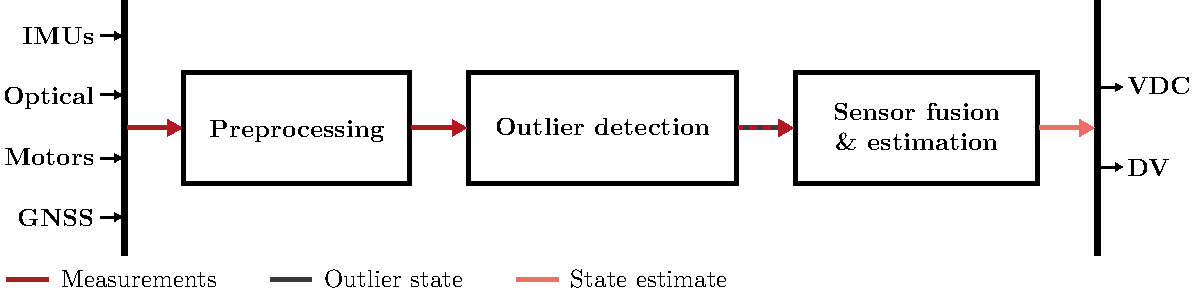
\includegraphics[width=\textwidth]{architecture_stateestimation}%
	\caption{Architecture of state estimation}
	\label{fig:architecture-stateestimation}
\end{figure}

A key feature is the unified mechanism for failure and sensor setup detection (requirements 2 and 3). Foundation is the realization that ultimately it does not matter if a measurement is unavailable due to an invalid signal or a missing sensor, therefore both cases can be treated the same. This allows a focused effort on a single component while reducing complexity. Still, the name \textit{failure detection} will be used. The following sections describe each of the three component in detail.


\subsection{Preprocessing}
Goal of the preprocessing stage is to harmonize all measurements and pre-fuse them for the subsequent estimation stage. Mostly, this is only a simple conversion to SI units, e.g., velocities from \si{\kilo\meter\per\hour} to \si{\meter\per\second}, or angles from \si{\deg} to \si{\radian}. Doing these conversions as early as possible simplifies subsequent computations and reduces error potential due to wrong units. For other signals, more preprocessing is necessary.

\begin{description}
\item[IMU] The most sophisticated preprocessing is required for the \glspl{imu}. The measurements are first rotated in three dimensions to correct any misalignment with the vehicle axes. This calibration must be performed every time the sensor orientation is changed. Then, we need a generic \gls{imu} fusion algorithm which can take an arbitrary number of sensors with known positions and fuse them into an estimate of the state variables $a_x$, $a_y$ and $\ddot{\psi}$ ($\dot{\psi}$ will be estimated in the last stage). An accurate estimate of these variables is important, because they are extensively used in the sensor fusion and performance components. This helps with reducing noise, but also enables calculation of the angular acceleration, which cannot be measured directly with our sensors. We always calculate the linear acceleration and angular velocity in three dimensions, and, in case of more than two \glspl{imu}, the angular acceleration as well. We provide two approaches for \gls{imu} fusion with the same interface, enabling drop-in replacement. Since the available \glspl{imu} need to be known at this point, performing the failure detection here instead of in the actual failure detection component is necessary.

The first approach fuses measurements by averaging, and is therefore called \textit{mean-based \gls{imu} fusion}. First, the angular velocity measurements from the gyrometers are averaged. Then, the angular accelerations are derived using equation \ref{eq:angacc-from-linacc-3d} from all combinations of two \glspl{imu} and averaged. For example, in the \gls{ev}, the combinations 1--2, 2--3 and 1--3 are regarded. In case only two \glspl{imu} are available, they are assumed to have a zero $z$-position and the angular acceleration is calculated using the simplified equation \ref{eq:angacc-from-linacc-2d}. In case only a single \gls{imu} is available, we assume $\alpha = \mathbb{0}$. Finally, the linear accelerations are transformed to the \gls{cog} using equation \ref{eq:offcenter-acceleration-3d} and averaged as well, which eliminates the effect of tangential and centripetal acceleration.

The second \textit{maximum-likelihood-based \gls{imu} fusion} approach is more sophisticated and is presented in \cite{Skog.2016}, with an extension proposed in \cite{Wahlstrom.2018}. The idea is to first find a maximum-likelihood estimate for $\omega$ given the linear acceleration and angular acceleration measurements of all sensors. This is done by solving a least-squares problem using the Gauss-Newton algorithm, with a fixed number of 10 iterations instead of checking for convergence. The maximum-likelihood estimate for $a$ and $\alpha$ is then as simple as plugging the previously found estimate into a linear equation.

\item[Optical velocity sensor] The optical cross-correlation velocity sensor is located on the right side behind the \gls{cog}, so its measurements need to be corrected to account for the component induced by a yaw rotation. Equation \ref{eq:offcenter-velocity-2d} is used to transform the measurements to the \gls{cog}. Note that the yaw rate is required, so a direct signal from the \gls{imu} preprocessing is required.

\item[\gls{gnss}] Position measurements from the \gls{gnss} arrive in latitude-longitude-height coordinates, but need to be transformed to topocentric east-north coordinates, i.e. coordinates on a plane tangential to the earth at a certain reference point~\cite[p.~475 f.]{Grewal.2007}. The transformation is based on the ellipsoid WGS 84 earth model used in \gls{gps} measurements. The reference point is the first known position, and all future positions will be represented in $x$-$y$-coordinates relative to the reference point.

Only speed measurements are available through \gls{gnss}, i.e. the absolute value of the velocity. However, since the vehicle sideslip angle $\beta$ is usually small and less than \SI{0.1}{\radian}, the longitudinal velocity can be approximated to be the speed, i.e. $v_x \approx \norm{v}$ and $v_y \approx 0$. This simplification works well in our design, since the \gls{gnss} speed will only be used for failure detection, not as part of the final state estimate. If separate measurements for the eastward and northward velocity become available, they can be transformed into vehicle coordinates using equation \ref{eq:transform-linear-velocity}. Note that this requires heading information, which might not always be available.

\item[Motor speed sensor] The motor rotation speeds are used as another vehicle velocity source via equation \ref{eq:wheelspeeds}, averaging over all four wheels to fuse them as described in section \ref{sec:motorspeeds-to-velocity}. Again, only the longitudinal velocity can be derived.
\end{description}


\subsection{Failure Detection}
Our approach towards failure detection is heavily based on the dual method presented in section \ref{sec:failure-types}, to help minimize both false-positives and false-negatives. The complete failure detection stage is shown in figure \ref{fig:architecture-failuredetection}. It receives signals from the preprocessing stage and determines the binary sensor state (OK, NOT OK), i.e. whether the sensor is available and does not contain failures. The target is to support one sensor failure, since more are unlikely.

\begin{figure}
	\centering
	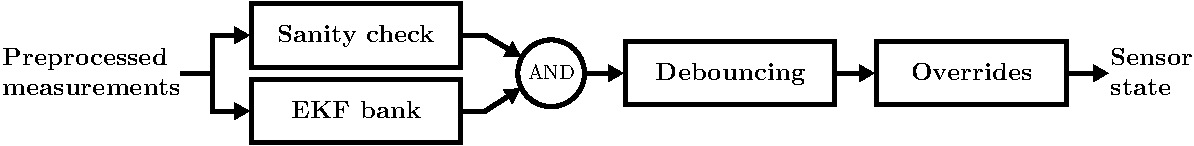
\includegraphics[width=\textwidth]{architecture_failuredetection}%
	\caption{Architecture of failure detection}
	\label{fig:architecture-failuredetection}
\end{figure}

Every input for the estimation stage undergoes a sanity check, presented in equations \ref{eq:failure-range} and \ref{eq:failure-maxchangerate}. This is also the failure detection method performed to select the \glspl{imu} for the \gls{imu} fusion. The range of the signal and the difference to the last sample are checked for plausibility, and the time since the last sample is used to detect a sensor timeout by means of a state machine. This is also the mechanism to detect the sensor setup, because missing sensors will timeout permanently and therefore be regarded as failure. While we described many other methods in section \ref{sec:failure-statisticalmethods}, we chose the simplest method with the least parameters.

Accurate knowledge of the vehicle velocity is of special importance for the performance component. Since we have three velocity sources, we can apply the \gls{ekf} bank approach from equation \ref{eq:failure-ekfbank}. We run three \glspl{ekf} in parallel using the model presented in the next section. For each \gls{ekf}, one sensor is disabled, so the other \glspl{ekf} generate high residuals in case of a failure of that sensor. This case is checked by comparing the normalized sum of squared residuals with a threshold. The covariance of all velocity measurements is identical to ensure equal weighting. This is necessary to detect persistent failures, since residuals caused by failures would otherwise quickly return to zero even if failures persist because the low-covariance measurements pull the estimate towards the faulty value. Note that successful fault isolation requires at least three measurements, otherwise only fault detection is possible. Because velocities are also checked by the \gls{ekf} bank, their plausibility check is configured to be rather lenient.

The results from the sanity check and the \gls{ekf} bank are logically and-ed, with OK for the results of non-velocities from the \gls{ekf} bank. Detected failures are then debounced to increase robustness in case failures appear and disappear quickly. Debouncing means that a signal is marked as NOT OK for a certain span of time after an failure has been detected, even if no failure is currently detected. Only if the time span passes without another failure, the signal is marked as OK once again. This logic is modeled using a state machine.

Last in the chain is a three-way override for each signal. Either the failure state can be directly forwarded, or forced to be OK or NOT OK. On the one hand, this allows to correct erroneous detection results, on the other hand it also provides a way to manually enable and disable sensors in case the sensor setup detection fails.

\subsection{EKF}
The final stage is the actual estimation of state variables. We use an \gls{ekf} for this task, since it is the standard and has been successfully applied in a lot of vehicles. Also, the system is not extremely non-linear, minimizing the potential benefits of using an \gls{ukf}. The linear acceleration and yaw acceleration are already estimated in the \gls{imu} fusion, so it remains to estimate the position, heading, velocity and yaw rate. While the yaw rate is already part of the \gls{imu} fusion, it can further be improved through correlation with the yaw acceleration. That is exactly what the \gls{ekf} is doing for all state variables as well: fusing available measurements which are corrected and correlated through a physical model.

To define the specific \gls{ekf} algorithm, we first need to set up the vectors shown in equation \ref{eq:design-ekf-vectors}. The state vector $x$ contains our variables to be estimated, the input vector $u$ contains variables that influence state propagation, and the measurement vector $z$ contains our sensor measurements.

\begin{subequations}\label{eq:design-ekf-vectors}
\begin{alignat}{2}%
x &= \begin{bmatrix}p_x\;, p_y,\; v_x,\; v_y,\; \psi,\; \dot{\psi}\end{bmatrix}^T \\%
u &= \begin{bmatrix}a_x,\; a_y,\; \ddot{\psi}\end{bmatrix}^T \\%
z &= \begin{bmatrix}p_{x,\textit{GNSS}},\; p_{y,\textit{GNSS}},\; v_{x,opt.},\; v_{y,opt.},\; v_{x,\textit{GNSS}},\; v_{x,motor},\; \psi_{\textit{GNSS}}, \dot{\psi}_{\textit{IMU}}\end{bmatrix}^T
\end{alignat}
\end{subequations}

Then we set up the process function to propagate the state vector and the measurement function to predict measurements. The process is defined by the system of differential equations shown in equation \ref{eq:design-ekf-process}, which describes the derivative of the state vector with respect to time. Therefore they constitute our physical model of the vehicle. It is a basic kinematic model which often works better than more sophisticated models like the non-linear single track model~\cite{AlexanderWischnewski.2019}. For an explanation of the equations for position and velocity, see sections \ref{sec:background-transform-linvelocity} and \ref{sec:background-cornering-acceleration}. It should be noted, that the lack of an initial heading, which is the case in the \gls{ev}, makes accurate prediction of the position next to impossible and also impairs the estimates of other state variables.

\begin{equation}\label{eq:design-ekf-process}%
\dot{x} = \frac{\partial x}{\partial t} (x, u)%
= \begin{bmatrix}\dot{x} \\ \dot{y} \\ \dot{v}_x \\ \dot{v}_y \\ \dot{\psi} \\ \ddot{\psi}\end{bmatrix}%
= \begin{bmatrix}v_x \cdot cos(\psi) - v_y \cdot sin(\psi) \\ v_x \cdot sin(\psi) + v_y \cdot cos(\psi) \\ a_x + \dot{\psi}v_y \\ a_y - \dot{\psi}v_x \\ \dot{\psi} \\ \ddot{\psi}\end{bmatrix}%
\end{equation}

To predict the current state, we use a forward Euler integration as shown in equation \ref{eq:design-ekf-predict}, which evaluates the current derivative and adds it to the previous state. This method works well for small time steps $\Delta t$, but a higher-order Runge--Kutta method might be necessary to guarantee numerical stability for larger time steps. 

\begin{equation}\label{eq:design-ekf-predict}%
\hat{x}_k^- = f(\hat{x}_{k-1}^+, u_k) = \hat{x}_{k-1}^+ + \Delta t \cdot \left. \frac{\partial x}{\partial t} \right|_{x = \hat{x}_{k-1}^+, u=u_k}%
\end{equation}

To propagate the covariance matrix, we need the Jacobian of the process function with respect to the state vector. Additionally, we need the process noise covariance, which is very hard to determine. Therefore we assume that process noise does not exist, but in exchange consider the uncertainty introduced by the measurements in the input vector, which are not considered in the standard \gls{ekf} equations. This is shown in equation \ref{eq:design-ekf-propagate-covariance}, which is adapted from equation \ref{eq:ekf-cov-propagation}. $I_6$ is the $6 \times 6$ identity matrix and $Q_k$ is the input covariance matrix. $F_k$ and $B_k$ are the discretized Jacobians of the process function with respect to the state vector and input vector, respectively. See appendix \ref{sec:appendix-ekf-equations} for the expanded forms of the process function's partial derivatives.

\begin{subequations}\label{eq:design-ekf-propagate-covariance}
\begin{alignat}{2}%
P_k^- &= F_k P_{k-1} F_k^T + B_k Q_k B_k^T \\%
F_k &= \frac{\partial f}{\partial x} = I_6 + \Delta t \cdot \left. \frac{\partial \dot{x}}{\partial x} \right|_{x = \hat{x}_{k-1}^+, u=u_k} \\%
B_k &= \frac{\partial f}{\partial u} = \Delta t \cdot \left. \frac{\partial \dot{x}}{\partial u} \right|_{x = \hat{x}_{k-1}^+, u=u_k}
\end{alignat}
\end{subequations}


The measurement function is just a linear function which maps state variables directly to their corresponding measurement prediction via the measurement matrix $H$ (see appendix \ref{sec:appendix-ekf-measurement}). Individual measurements can be enabled and disabled using the binary measurement mask $m$, which is turned into a diagonal matrix. The mask is based on the sensor state from the failure detection. Additionally, for sensors which do not send data at the rate that the \gls{vdc} is executed, measurements are only enabled when new data arrive
. For this, we check if the time since the arrival of the last measurement is less than in the previous execution of the \gls{vdc}. Furthermore, \gls{gnss} velocity measurements are only enabled if the other velocity sources are unavailable, since its delay in dynamic situations impairs the estimate.

\begin{equation}
\hat{z} = \textit{diag}(m) H \hat{x}
\end{equation}

The same measurement mask is also applied to the real measurements and the residual. Furthermore, we normalize the predicted and measured heading to be between $-\pi$ and $\pi$. Other than that, the correction stage of the \gls{ekf} uses exactly the equations described in \ref{sec:background-ekf}. Since the \gls{ekf} works iteratively, the state vector and its covariance matrix need to be stored between iterations. Before the first iteration, the state vector is is initialized with zeros and its covariance matrix is set to the identity matrix.
